\section{Introduction}

As has been pointed out by the incident at the Ketelbrug between Emmeloord and Lelystad, bridges require a very precise control system.  Many examples exist where bridges are not opened or closed properly, where bridge components break down or the bridge is being stuck in a particular state. The goal of this project is to design a safety layer that can be added to the main control interface, in order to capture all possible situations and failures.

In order to achieve this, we first define all requirements that must be met by the bridge. This is being done both informally and formally using $\mu$-calculus, a way of expressing modal logic. Then, we model the bridge using mCRL2, a tool to create concurrent discrete event systems. Within this program, the $\mu$-calculus requirements can be verified on whether they are being satisfied. This is step and will result in an verification overview of all the requirements of our bridge. After this, we will make the model open to user input by verifying the safety for all actions in each state. By doing this, the system also covers the realistic event of the bridge operator interrupting the system.

Modeling the bridge can be done in various levels of detail. For our model, we make use of the following assumptions:
%
\begin{itemize}
	\item	The individual objects of a particular components (sign, barrier or lock) operate (for now) as one identical object (so they always have the same status)
	\item When the majority of the sensors have determined a particular state, the object is said to be in that state (e.g. if three or four sensors detect the bridge deck to be open, the bridge can be considered open)
	\item If a communication has been established between two objects, it means that a \texttt{send} action from object A has been received, processed and confirmed by the majority of the sensors of object B
	%\item If three or four sensors detect an open/closed bridge, the bridge can be considered open/closed
	%\item If the four sensors	 have a 50/50 detection on the bridge deck, the bridge should remain in its current position (open/closed)
	%\item A barrier can only be considered to be down when the majority of the sensors detect a lowered barrier
\end{itemize}
%
In the next subsection, the desired behaviour of the bridge is being determined and defined. Section \ref{sec:glob} contains the global requirements that will be met in our system. Specific interactions that can be performed by the bridge are discussed in Section \ref{sec:act}, whereas section \ref{sec:arch} discusses the used architecture of the system. In section \ref{sec:trans} the requirements stated earlier are translated into these interactions. The modeling of the bridge is covered by section \ref{sec:model}, followed by section \ref{sec:check} holding the results of the system validation. Finally, the conclusion can be found in section \ref{sec:conclusion}.

\subsection{Desired behavior of the bridge}

Although it seems pretty straightforward what should be the desired behavior of a bridge, the Ketelbrug accident shows us that this can be slightly more complicated that it appears. For the project, the Project Guide\footnote{J. J. A. Keiren, System Validation (IN4387) Project Guide, VU University Amterdam, november 2013} has described the desired behavior in detail. For the sake of the clarity of this report, the general outline is repeated here. The bridge has two main functions: open en close. The sequence below shows all steps that need to be taken to open and to close the bridge.
%
\begin{table}[h]%
\begin{tabular}{l}
	\footnotesize
	\texttt{switch on pre signs -> switch on stop signs -> lower barriers -> disengage deck locks -> lift bridge deck}\\
\end{tabular}
\caption{}
\label{}
\end{table}
%
\begin{table}[h]%
\begin{tabular}{l}
	\footnotesize
	\texttt{lower bridge deck -> engage deck locks -> raise barriers -> switch off stop signs -> switch off pre signs}\\
\end{tabular}
\caption{}
\label{}
\end{table}
%
The most important feature is that every action can only be performed when the previous action has already occurred properly (according to assumptions we stated earlier). For example, it undesireable for cars to have a barrier coming down when no warning sign has been switched on previously. Also, the system has to be free of deadlocks. 

In the following sections of the report, the bridge components will be labelled with individual identifiers. These are based on figure \ref{fig:setup}, an image from the project guide. 
%
\begin{figure}[htb]%
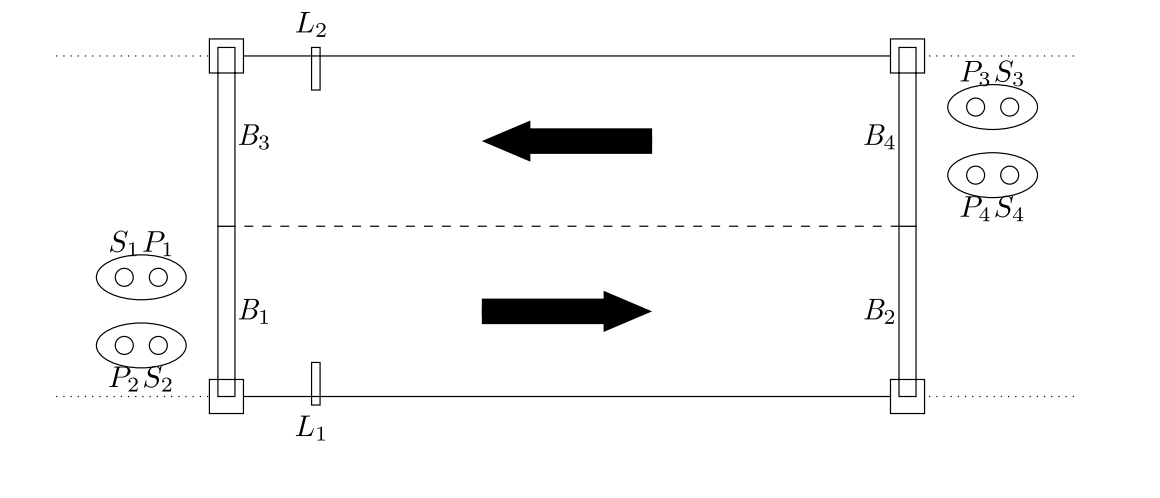
\includegraphics[width=\columnwidth]{Images/Setup.png}%
\caption{Setup of the bridge, using labelled components (from: Project Guide)}%
\label{fig:setup}%
\end{figure}
%

\newpage